%%%%% Chapter 3
\documentclass[../thesis.tex]{subfiles}
\begin{document}

\chapter[Reducing stranded assets in the Indian power sector]{\textit{Reducing stranded assets through early action in the Indian power sector}\raisebox{.3\baselineskip}{\normalsize\footnotemark}\footnotetext{%
    published in \emph{Environmental Research Letters} as
  Malik, A., Bertram, C., Despres, J., Emmerling, J., Fujimori, S., Garg, A., Kriegler, E., Luderer, G., Mathur, R., Roelfsema, M., Shekhar, S., Vishwanathan, S., Vrontisi, Z. (2020). Reducing stranded assets through early action in the Indian power sector. Environmental Research Letters, 15(9), 094091. https://doi.org/10.1088/1748-9326/ab8033}}\label{ch:ERLPaper}
  
  
\bigskip {\raggedleft \em
Aman Malik\\
Christoph Bertram\\
Jacques Despres\\
Johannes Emmerling\\
Shinichiro Fujimori\\
Amit Garg\\
Elmar Kriegler\\
Gunnar Luderer\\
Ritu Mathur\\
Mark Roelfsema\\
Swapnil Shekhar\\
Saritha Vishwanathan\\
Zoi Vrontisi\\
}
\cleardoublepage
\includepdf[scale=0.92,offset= 0 -3mm,
  pages=2-,fitpaper=false, 
%  addtotoc={%   
%  2, subsection,    2, Introduction,		             p3s2,
%  3, subsection,    2, Methods,		 p3s2,
%  5, subsection,    2, Results,	 p3s3,
%  10, subsection,   2, Discussion,  p3s4,
%  12, subsection,   2, Conclusions,p3r}
   pagecommand={\thispagestyle{fancy}}]{pdfs/malik2020_erl.pdf}
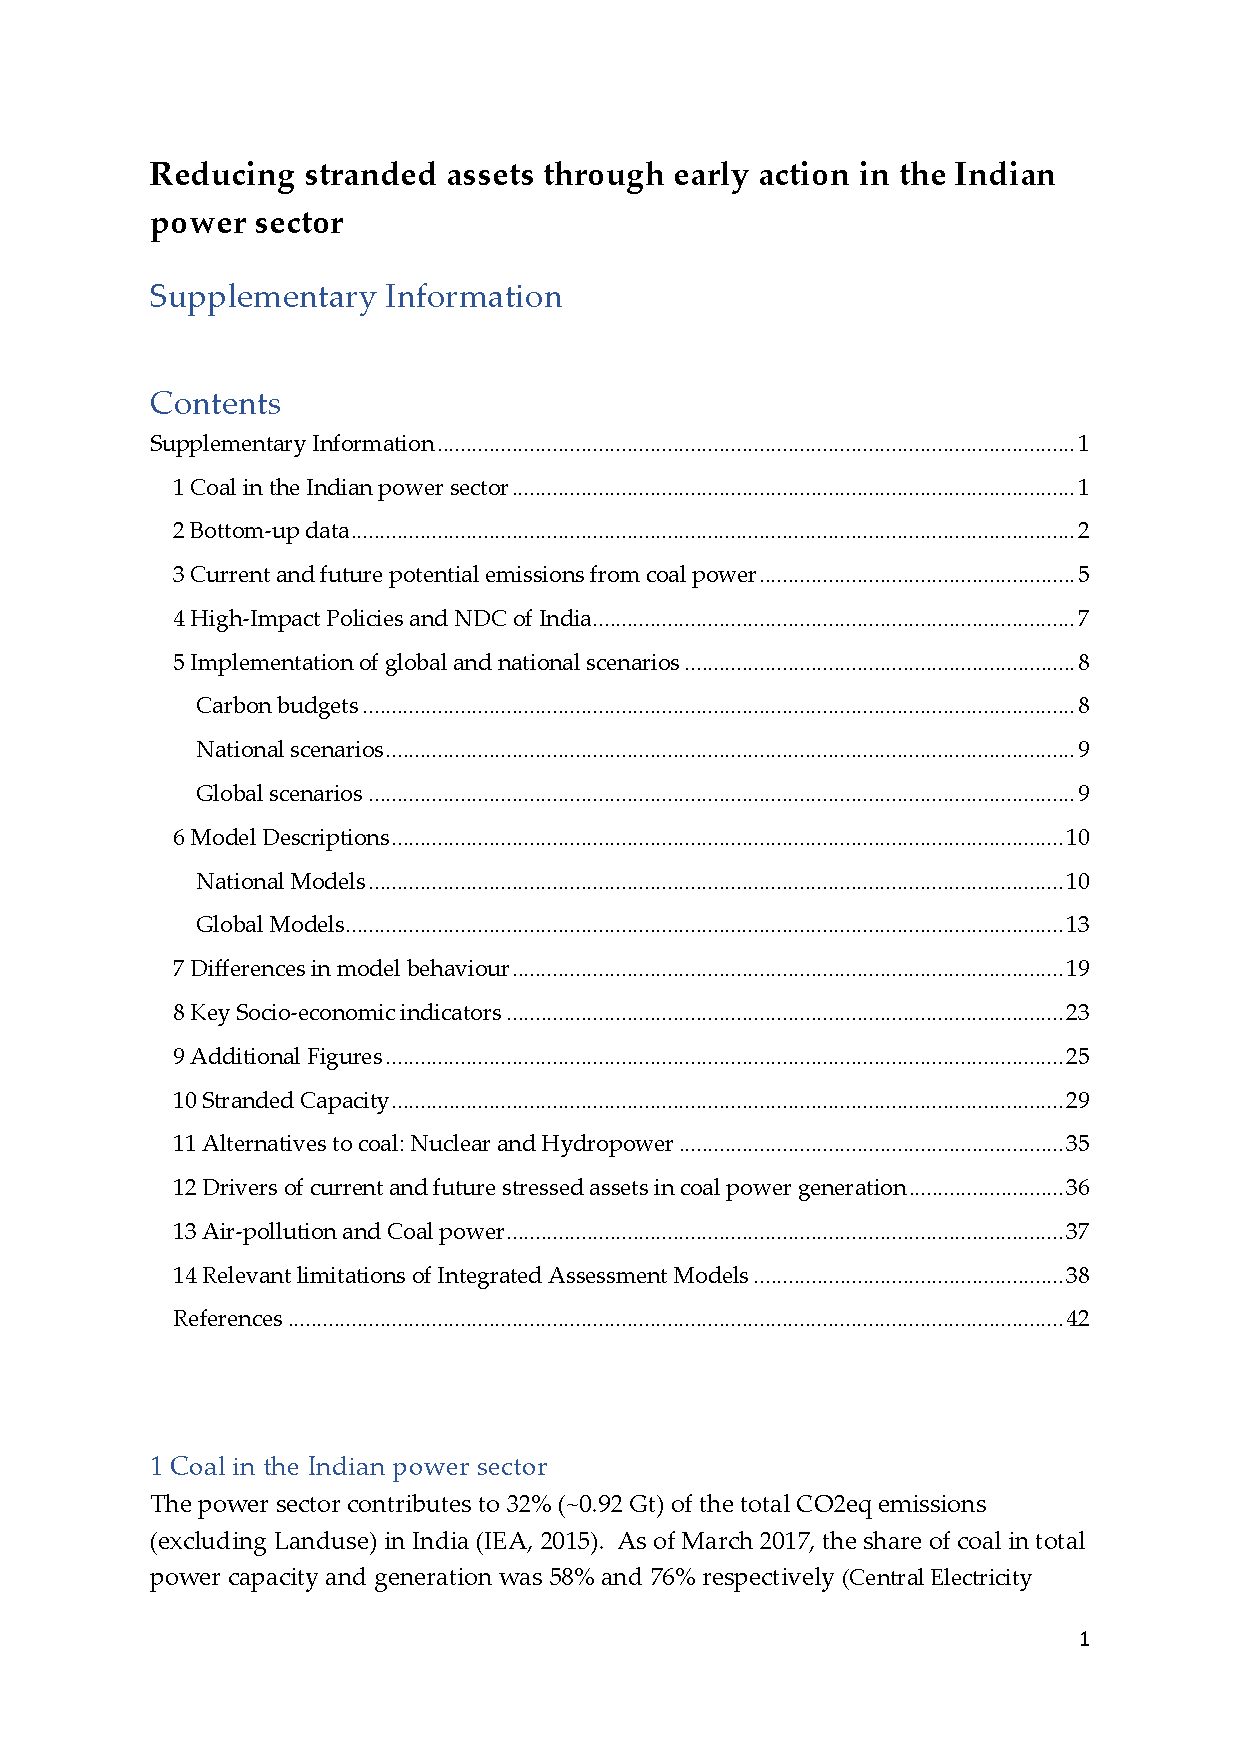
\includepdf[pages=-, 
%addtotoc={%   
%  1, subsection,    2, Supplementary	Information,		                        p3sm},
  pagecommand={}]{pdfs/malik2020_erl_si.pdf}

\clearpage
\end{document}